% -*-coding: latin-9;-*-

% Not all the slides here are shown, but keep them for other presentations
\let\ifPresentHiddenSlides=\iffalse

% For Ubuntu 22.04, it looks like the
% xcolor={dvipsname,svgnames,x11names} is not enough to have color
% Coral
\PassOptionsToPackage{dvipsname,svgnames,x11names}{xcolor}


%% To deal with the colors and number of slides per page according to the
%% \VersionPapier switch :
\ifx\VersionExpose\UnTrucInexistant%

% The handout version
\documentclass[aspectratio=169,handout,compress,10pt,hyperref={hyperindex},xcolor={dvipsname,svgnames,x11names}]{beamer}
\usepackage{pgfpages}
\pgfpagesuselayout{4 on 1}[a4paper,landscape,border shrink=5mm]
\else
% The slide version
\documentclass[aspectratio=169,compress,10pt,hyperref={hyperindex},xcolor={dvipsname,svgnames,x11names}]{beamer}
\fi

\usepackage[latin9]{inputenc}

\usepackage{header_SYCL}

% Some specialization according to the official AMD 2022 PowerPoint
% template
\usepackage{beamer_AMD_2022}

% To add arrows between slide pieces:
% Here because of catcode wizardy I guess :-(
% Should go into tikz_hpc
% Could use \pgftext instead of using "text depth=0pt"
\newcommand{\PlaceTextNode}[2]{\tikz{\node[inner sep=0pt,text depth=0pt] (#1) {#2};}}

% To decorate some lstlisting lines:
\usepackage{balloon_rk}

% Use SYCL+OpenCL as the default language
\lstset{language=SYCL,showstringspaces=false,
  basicstyle=\small}

%\tracingall

\author[]{Ronan Keryell (\url{ronan.keryell@amd.com})}

\title[Advanced SYCL Techniques and Best Practices]{SYCL introduction}

\subtitle{Advanced SYCL Techniques and Best Practices}

\date{2023/05/30 @ NERSC}

\institute[\copyright{} Copyright 2023 Khronos]{Fellow Software
  Development Engineer @ AMD Research \& Advanced Development\\
  % San Jos�, California\\
  Khronos SYCL specification editor \& ISO C++ committee member}

\pgfdeclareimage[width=0.8cm]{logo-SYCL}{Khronos/Logos/SYCL/SYCL_500px_June16}
\logo{\hbox to 0.75cm{\vbox{%
      \href{https://www.khronos.org/sycl}{\pgfuseimage{logo-SYCL}}}}}


\begin{document}

\SetImageBackground{Background/Khronos-background-16-9}
{
  %\SetImageBackground{Background/AMD/Corporate_Template/Presentations_Templafy/Corporate_PPT_Template-White_Background-6x9-title_page-23.pdf}

  \begin{frame}[plain]
%\tracingall=1
    \titlepage
%\tracingall=0
  \end{frame}
}



\begin{frame}{Typical modern/future system}
  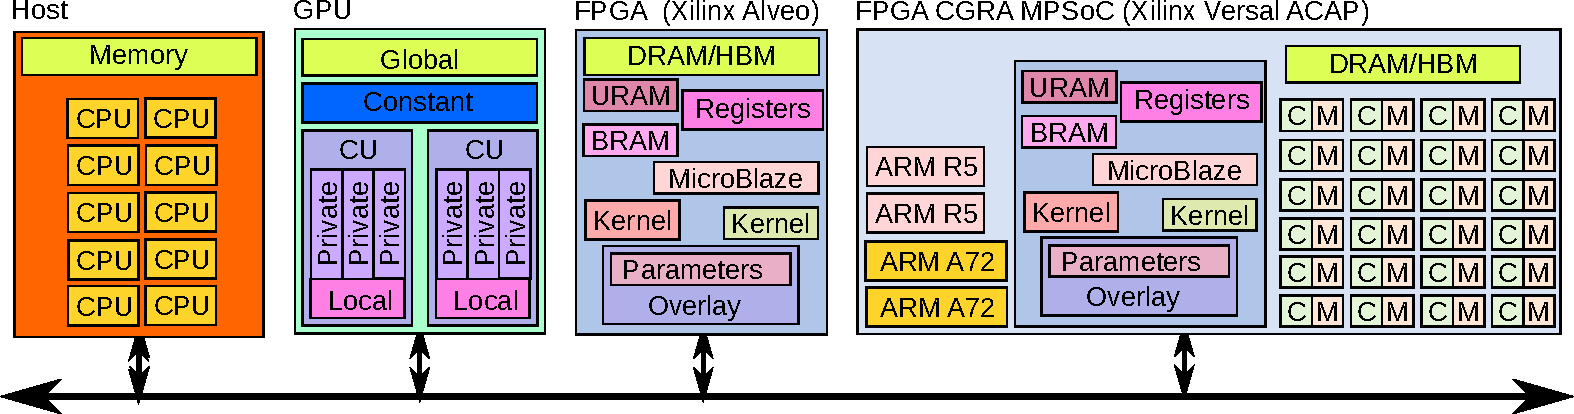
\includegraphics[width=\textwidth]{Images/ordinateurs/Accelerators/System_View/host_with_Xilinx_platforms}

  \begin{itemize}
  \item<+-> Add your own accelerator to this picture...
  \item<+-> Scale this from embedded system to data-center/HPC level\ldots
  \item<+-> Chiplet revolution allows mix-and-match in package
  \item<+-> Need a programming model for the \emph{full} system\ldots
  \item<+-> Tim Mattson's law: no new language! \smiley
  \end{itemize}
\end{frame}




\begin{frame}{Remember C++ ?}
  \begin{BoiteA}{2-line description by Bjarne Stroustrup}
    \begin{itemize}
    \item Direct mapping to hardware
    \item Zero-overhead abstraction
    \end{itemize}
  \end{BoiteA}
\end{frame}


\begin{frame}[fragile]{Modern Python/C/Modern C++/Old C++}
  \begin{multicols}{2}
    \begin{itemize}
    \item Python 3.11
      \begin{lstlisting}[language=Python]
v = [ 1, 2, 3, 5, 7 ]
print(v)
      \end{lstlisting}
      \url{https://godbolt.org/z/Kq9vc1jhY}
    \item C99 (also usable in C++)
      \begin{lstlisting}
#include <stdio.h>
int a[] = { 1, 2, 3, 5, 7 };
for (int i = 0;
     i < sizeof(a)/sizeof(a[0]);
     ++i)
  printf("%d ", a[i]);
      \end{lstlisting}

      \columnbreak

    \item C++23
      \begin{lstlisting}
import std;
std::vector v { 1, 2, 3, 5, 7 };
std::println("{}", v);
      \end{lstlisting}
    \item C++03
      \begin{lstlisting}
#include <iostream>
#include <vector>
std::vector<int> v;
v.push_back(1);
v.push_back(2);
v.push_back(3);
v.push_back(5);
v.push_back(7);
for (std::vector<int>::iterator i =
       v.begin(); i != v.end(); ++i)
  std::cout << *i << std::endl;
      \end{lstlisting}
    \end{itemize}
  \end{multicols}
\end{frame}


\begin{frame}
  \Huge
  \begin{center}
    But...\\
    No heterogeneous computing in C++\\
    \frownie
  \end{center}
\end{frame}


\SlideFromImageFile{Khronos/Members/Khronos Member Logo Field}

\SlideFromImageFile{About_Khronos_Slide-2018}



\begin{frame}{SYCL 2020 from Khronos Group, published on 2021-02-09}
%[height=0.95\textheight]
  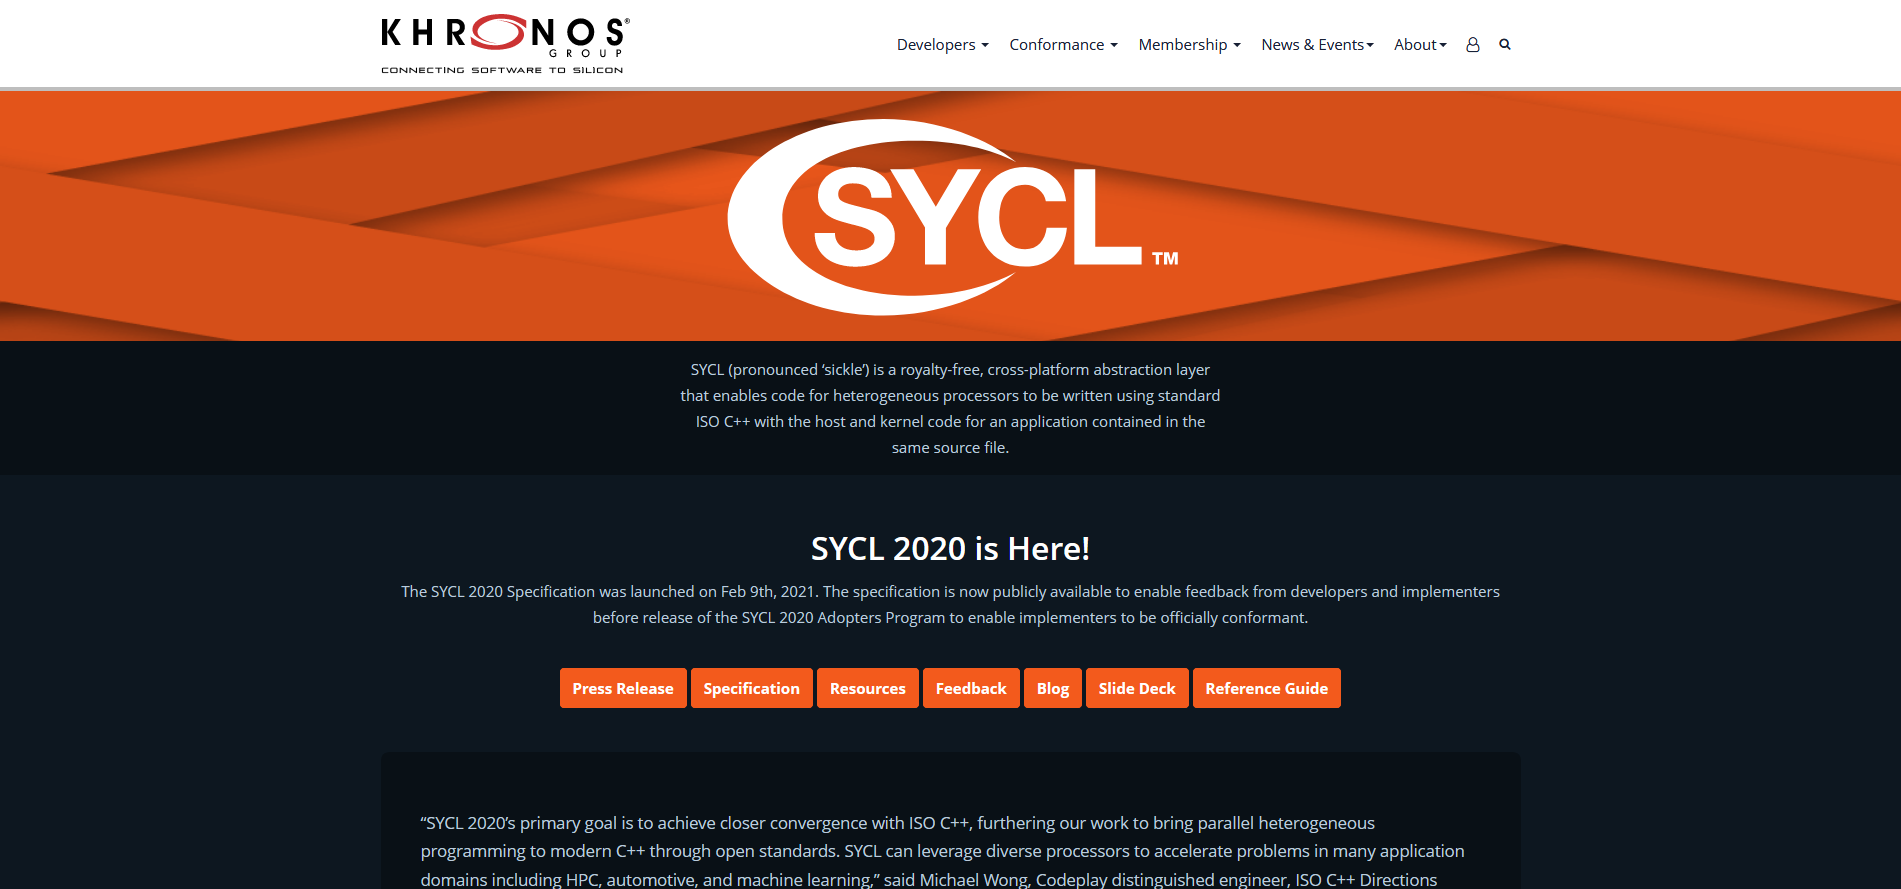
\includegraphics[width=\textwidth]{Languages/SYCL/Specification/Screenshot_2021-06-11 SYCL - C++ Single-source Heterogeneous Programming for Acceleration Offload}

  \begin{itemize}
  \item \url{https://www.khronos.org/sycl}
  \end{itemize}
\end{frame}




\begin{frame}{SYCL ecosystem is growing}
  \centerline{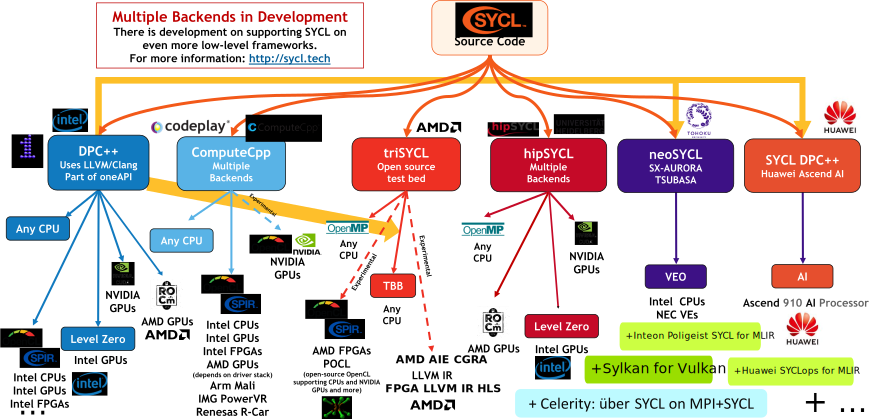
\includegraphics[height=0.8\textheight]{Images/Languages/SYCL/Implementations/SYCL-ecosystem-2023-04-13}}
  \url{https://www.khronos.org/blog/sycl-2020-what-do-you-need-to-know}
\end{frame}


\begin{frame}[fragile]{SYCL 2020 $\equiv$ heterogeneous simplicity with modern C++}
  % Add the descriptive boxes
  \begin{tikzpicture}[remember picture, overlay]
    \scriptsize
    \node<2-> [
      xshift=-0.3\paperwidth,
      yshift=-0.1\paperheight,
      anchor=north east
    ](bufferNode)
    at (current page.north east)
    {
      \scriptsize
      \begin{BoiteA}[width=0.33\hsize]{Abstract storage}
        \begin{itemize}
        \item Host or device (remote) memory
        \end{itemize}
      \end{BoiteA}
    };

    \node<3-> [
      %xshift=-0.1\paperwidth,
      yshift=-0.25\paperheight,
      anchor=north east
    ](kernelNode)
    at (current page.north east)
    {
      \scriptsize
      \begin{BoiteA}[width=0.33\hsize]{Code executed on device (``kernel'')}
        \begin{itemize}
        \item ``Single-source''
        \item Seamless integration in host code
        \item Type-safety
        \item Asynchronous execution
        \end{itemize}
      \end{BoiteA}
    };

    \node<4-> [
      %xshift=0.25\paperwidth,
      yshift=0.05\paperheight,
      anchor=south east
    ](accessorNode)
    at (current page.south east)
    {
      \scriptsize

      \begin{BoiteA}[width=0.38\hsize]{Accessor}
        \begin{itemize}
        \item Express access intention
        \item Implicit data flow graph
        \item Automatic data transfers across devices
        \item Overlap computation \& communication
        \end{itemize}
      \end{BoiteA}
    };
    \node<5-> [
      xshift=-0.05\paperwidth,
      yshift=-0.1\paperheight,
      anchor=north west
    ](queueNode)
    at (current page.north west)
    {
      \scriptsize

      \begin{BoiteA}[width=0.32\hsize]{Queue}
        \begin{itemize}
        \item Direct work to specific accelerator
        \item Submission of a command group
        \end{itemize}
      \end{BoiteA}
    };
    % Add arrows from boxes too source code
    \draw<2-> [overlay,->,very thick,red] (node cs:name=bufferNode) to (pic cs:buffer);
    \draw<3-> [overlay,->,very thick,red] (node cs:name=kernelNode) to (pic
      cs:kernel);
    \draw<3-> [overlay,-,line width=6mm,yellow] (pic cs:kernelStart) to (pic cs:kernel);
    \draw<4-> [overlay,->,very thick,red] (node cs:name=accessorNode) to (pic cs:accessor);
    \draw<4-> [overlay,->,very thick,red] (node cs:name=accessorNode) to (pic cs:hostAccessor);
    \draw<5-> [overlay,->,very thick,red] (node cs:name=queueNode) to (pic cs:queue);
  \end{tikzpicture}
  \begin{lstlisting}[name=SYCLsample]
#include <iostream>
#include <sycl/sycl.hpp>
constexpr int n = 32;

int main () {
  sycl::buffer<int> buf�\tikzmark{buffer}� { n };
  sycl::�\tikzmark{queue}�queue {}.submit([&](auto &h) {
      sycl::accessor a { buf, h, sycl::write_only, sycl::no_init }�\tikzmark{accessor}�;
      h.parallel_for(n, �\tikzmark{kernelStart}�[=](auto i) { a[i] = i; }�\tikzmark{kernel}�);
  });
  for (sycl::host_accessor a { buf }�\tikzmark{hostAccessor}�; auto e : a)
      std::cout << e << std::end;
}
  \end{lstlisting}
\end{frame}


\begin{frame}[fragile]{SYCL 2020 with unified shared memory (USM)}
  \begin{multicols}{2}
    \begin{lstlisting}[basicstyle=\scriptsize]
// Using buffers and accessors

#include <iostream>
#include <sycl/sycl.hpp>

constexpr int n = 32;

int main () {
 sycl::buffer<int> buf { n };

 sycl::queue {}.submit([&](auto &h) {
  sycl::accessor a { buf, h, sycl::write_only,
                     sycl::no_init };
  h.parallel_for(n, [=](auto i) { a[i] = i; });
 });

 for (sycl::host_accessor a { buf }; auto e : a)
  std::cout << e << std::endl;
}

// Using USM only

#include <iostream>
#include <sycl/sycl.hpp>

constexpr int n = 32;

int main () {
 sycl::queue q;
 int* a = sycl::malloc_shared<int>(n, q);

 q.parallel_for(n, [=](auto i) { a[i] = i; });
 q.wait();

 for (int i = 0; i < n; i++)
  std::cout << a[i] << std::endl;

 sycl::free(a, q);
}
    \end{lstlisting}
  \end{multicols}
\end{frame}



\begin{frame}[fragile]{Matrix addition as implicit task graph programming}
  \vspace{-.75cm}
  \begin{multicols}{2}
    % Put it before to avoid overriding the listing
    \balloono{comment}{TaskGraph}{18}{27}
    \balloon{comment}{TaskGraph}{23}{26}
    % Adjust for the column break, because it is not compatible with
    \balloono{comment}{TaskGraph}{30}{35}
    % Repeat after the column break
    \balloono{comment}{TaskGraph}{40}{45}
    % Adjust for the column break, because it is not compatible with
    \balloon{comment}{TaskGraph}{41}{44}
    \balloono{comment}{TaskGraph}{47}{60}
    \balloon{comment}{TaskGraph}{56}{59}
    \begin{tikzpicture}[remember picture,overlay]
      \draw [overlay,->,very thick,red] (pic cs:PA) to[bend left] (pic cs:CA);
      \draw [overlay,->,very thick,red] (pic cs:PB) to[bend left] (pic cs:CB);
      \draw [overlay,->,very thick,red] (pic cs:PC) to[bend right] (pic cs:CC);
    \end{tikzpicture}
    % triSYCL/tests/examples/demo_parallel_matrices_add.cpp
    \begin{lstlisting}[basicstyle=\tiny,name=TaskGraph]
#include <sycl/sycl.hpp>
#include <iostream>
// Size of the matrices
constexpr size_t n = 2000;
constexpr size_t m = 3000;
int main() {
 // Create a queue to work on default device
 sycl::queue q;
 // Create some 2D buffers of float for our matrices
 sycl::buffer<double, 2> a({ n, m });
 sycl::buffer<double, 2> b({ n, m });
 sycl::buffer<double, 2> c({ n, m });

 // Launch a first asynchronous kernel to initialize a
 q.submit([&](auto& cgh) {
   // The kernel write a, so get a write accessor on it
   sycl::accessor A�\tikzmark{PA}� { a, cgh, sycl::write_only, sycl::no_init };

   // Enqueue parallel kernel on a n*m 2D iteration space
   cgh.parallel_for<class init_a>({ n, m },
                      [=] (sycl::id<2> index) {
                        A[index] = index[0]*2 + index[1];
                      });
 });

 // Launch an asynchronous kernel to initialize b
 q.submit([&](auto& cgh) {
   // The kernel write b, so get a write accessor on it
   sycl::accessor B�\tikzmark{PB}� { b, cgh, sycl::write_only, sycl::no_init };
   /* From the access pattern above, the SYCL runtime detect
      this command_group is independant from the first one
      and can be scheduled independently */




   // Enqueue a parallel kernel on a n*m 2D iteration space
   cgh.parallel_for<class init_b>({ n, m },
                      [=] (sycl::id<2> index) {
                        B[index] = index[0]*2014 + index[1]*42;
                      });
 });
 // Launch an asynchronous kernel to compute matrix addition c = a + b
 q.submit([&](auto& cgh) {
   // In the kernel a and b are read, but c is written
   sycl::accessor �\tikzmark{CA}�A { a, cgh, sycl::read_only };
   sycl::accessor �\tikzmark{CB}�B { b, cgh, sycl::read_only };
   sycl::accessor �\tikzmark{PC}�C { c, cgh, sycl::write_only, sycl::no_init };
   // From these accessors, the SYCL runtime will ensure that when
   // this kernel is run, the kernels computing a and b completed

   // Enqueue a parallel kernel on a n*m 2D iteration space
   cgh.parallel_for<class matrix_add>({ n, m },
                                  [=] (sycl::id<2> index) {
                                    C[index] = A[index] + B[index];
                                  });
 });
 /* Request an access to read c from the host-side. The SYCL runtime
    ensures that c is ready when the accessor is returned */
 sycl::host_accessor �\tikzmark{CC}�C { c };
 std::cout << std::endl << "Result:" << std::endl;
 for(size_t i = 0; i < n; i++)
   for(size_t j = 0; j < m; j++)
     // Compare the result to the analytic value
     if (C[i][j] != i*(2 + 2014) + j*(1 + 42)) {
       std::cout << "Wrong value " << C[i][j] << " on element "
                 << i << ' ' << j << std::endl;
       exit(-1);
     }
 std::cout << "Good computation!" << std::endl;
 return 0;
}
    \end{lstlisting}
  \end{multicols}
\end{frame}


\begin{frame}{Asynchronous task graph model}
  \begin{itemize}
  \item Theoretical graph of an application described \emph{implicitly}
    with kernel tasks using buffers through accessors

    \medskip

    \includegraphics[width=\hsize]{Pictures/unscheduled_task_graph-2020}

  \item Possible schedule by SYCL runtime:

    \centerline{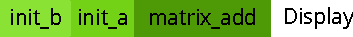
\includegraphics[width=0.4\hsize]{Pictures/scheduled_task_graph}}

    \item[\vavers] Automatic overlap of kernels \& communications
      \begin{itemize}
      \item No need for complex events and queue management
      \item Even better when looping around in an application
      \item Assume it will be translated into pure back-end event graph
      \item Runtime uses as many threads \& back-end queues as necessary
      \end{itemize}
  \end{itemize}
\end{frame}




\begin{frame}[fragile]{Other SYCL features}
  \alert{*} $\equiv$ In this tutorial
  \begin{multicols}{2}
    \begin{itemize}
    \item \alert{In-order queue}
    \item \alert{Multi-devices}
    \item \alert{Atomic references}
    \item \alert{Reductions}
    \item \alert{Work-group and sub-group algorithms}
    \item \alert{Work-group local memory}
    \item \alert{Events}
    \item Properties
    \item Aspects
    \item Images
    \item \alert{Small vectors} (\lstinline|sycl::vec| \& %
      \lstinline|sycl::marray|)
    \item Multi-pointers
    \item Kernel bundles
    \item Specialization constants
    \item Error handling
    \item Library functions
    \item Back-ends
    \item Interoperability
    \item \ldots
    \end{itemize}
  \end{multicols}
\end{frame}


\begin{frame}[fragile]{21 lines of heterogeneous serendipity on my desktop}
  {\tiny\url{https://github.com/triSYCL/sycl/blob/sycl/unified/next/sycl/test/vitis/disabled/inclusive_devices.cpp}}
  \begin{lstlisting}[basicstyle=\scriptsize]
#include <iostream>
#include <sycl/sycl.hpp>
int main() {
  sycl::buffer<int> v { 10 };
  auto run = [&] (auto device_name, auto work) {
    sycl::queue { [&](sycl::device dev) {
      return (device_name == dev.template get_info<sycl::info::device::name>()) - 1;
    } }.submit([&](auto& h) {
      auto a = sycl::accessor { v, h };
      h.parallel_for(a.size(), [=](int i) { work(i, a); });
    });
  };
  run("Intel(R) Xeon(R) CPU E5-2630 v4 @ 2.20GHz", [](auto i, auto a) { a[i] = i; });
  run("Quadro P400", [](auto i, auto a) { a[i] = 2 * a[i]; });
  run("Intel(R) FPGA Emulation Device", [](auto i, auto a) { --a[i]; });
  run("AMD Radeon VII", [](auto i, auto a) { a[i] = a[i] * a[i]; });
  run("xilinx_u200_gen3x16_xdma_base_1", [](auto i, auto a) { a[i] += + 3; });
  for (auto e : sycl::host_accessor { v })
    std::cout << e << ", ";
  std::cout << std::endl;
}
  \end{lstlisting}

  \tiny \texttt{\$DPCPP\_HOME/llvm/build/bin/clang++ -std=c++2b -fsycl -fsycl-targets=spir64\_x86\_64,nvptx64-nvidia-cuda,amdgcn-amd-amdhsa,fpga64\_hls\_hw,spir64\_fpga -Xsycl-target-backend=amdgcn-amd-amdhsa --offload-arch=gfx906 -Xsycl-target-backend=nvptx64-nvidia-cuda --offload-arch=sm\_61 inclusive\_devices.cpp -o inclusive\_devices}

  \begin{tikzpicture}[remember picture, overlay]
    \scriptsize
    \node<2-> [
      %xshift=-0.3\paperwidth,
      yshift=-0.1\paperheight,
      anchor=north east
    ](bufferNode)
    at (current page.north east)
    {
      \scriptsize
      \begin{minipage}[c]{0.4\linewidth}
        \begin{itemize}
        \item No \texttt{template} or \texttt{typename} or
          \texttt{class} or\ldots \smiley
        \item No extension or attribute or\ldots \smiley
        \item Generic \& type-safe
        \item No explicit data motion or boiler-plate code
        \item Different accelerators/vendors in same program!
        \end{itemize}
      \end{minipage}
    };
  \end{tikzpicture}
\end{frame}


\begin{frame}{Inclusive heterogeneous computing with SYCL\ldots}
  No transistors left behind!
\end{frame}



\begin{frame}{Some of the existing SYCL back-ends}
  \centerline{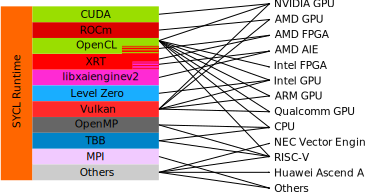
\includegraphics[height=0.8\textheight]{Images/Languages/SYCL/Implementations/sycl_rt_backend_hardware}}
\end{frame}


\begin{frame}{Unique SYCL feature: interoperability with backends}
  \begin{itemize}
  \item Porting existing code
    \begin{itemize}
    \item Code already based on OpenCL/CUDA/OpenMP/HIP/\ldots{} (or
      whatever backend)
    \item Want to change just part of application to use SYCL
    \end{itemize}
  \item Incorporating a backend module into a SYCL application
    \begin{itemize}
    \item Application based on SYCL
    \item Want to call some OpenCL/CUDA/OpenMP/HIP/\ldots{} library
      (or whatever backend)
    \end{itemize}
  \item Take advantage of backend-specific features
  \item Disadvantage: reduces portability!
    \begin{itemize}
    \item Not all implementations may support your backend
    \end{itemize}
  \item[\vavers] Unique feature of SYCL!
  \end{itemize}

  {\scriptsize
    %% IWOCL and SYCLcon 2022
    %% Using Interoperability Mode in SYCL 2020
    Aksel ALPAY, Thomas APPLENCOURT, Gordon BROWN, Ronan KERYELL and
    Gregory LUECK. ``Using interoperability mode in SYCL 2020.'' In
    SYCLcon 2022: International Workshop on SYCL. Association for
    Computing Machinery, May 2022. doi:10.1145/3529538.3529997.
    \url{https://www.iwocl.org/wp-content/uploads/39-presentation-iwocl-syclcon-2022-aksel.pdf}
    \url{https://www.youtube.com/watch?v=XIPhuesdqYE}
  }
\end{frame}


\begin{frame}[fragile]{Type 1: SYCL object from backend object}
  \framesubtitle{``Higher-level XRT'' for AMD FPGA in 43 lines with SYCL}
  \begin{multicols}{2}
    \begin{lstlisting}[basicstyle=\tiny]
#include <cassert>
#include <sycl/sycl.hpp>
#include <sycl/ext/xilinx/xrt.hpp>
#include <xrt.h>
#include <xrt/xrt_kernel.h>
constexpr int size = 4;
int main() {
  sycl::buffer<int> a { size };
  sycl::buffer<int> b { size };
  sycl::buffer<int> c { size };
  {
    sycl::host_accessor a_a { a };
    sycl::host_accessor a_b { b };
    for (int i = 0; i < size; ++i) {
      a_a[i] = i;
      a_b[i] = i + 42;
    }
  }
  sycl::queue q;
  xrt::device xdev =
    sycl::get_native<sycl::backend::xrt>(q.get_device());
  xrt::kernel xk { xdev, xdev.load_xclbin("vadd.hw_emu.xclbin"),
                   "vadd" };
  sycl::kernel k
    { sycl::make_kernel<sycl::backend::xrt>(xk, q.get_context()) };

  q.submit([&](sycl::handler& cgh) {
    cgh.set_args(sycl::accessor { a, cgh, sycl::read_only },
                 sycl::accessor { b, cgh, sycl::read_only },
                 sycl::accessor { c, cgh, sycl::write_only,
                                  sycl::no_init },
                 size);
    cgh.single_task(k);
  });
  {
    sycl::host_accessor a_a { a };
    sycl::host_accessor a_b { b };
    sycl::host_accessor a_c { c };
    for (int i = 0; i < size; ++i) {
      int res = a_a[i] + a_b[i];
      int val = a_c[i];
      assert(val == res);
    }
  }
}
    \end{lstlisting}
  \end{multicols}
  {\tiny\url{https://github.com/keryell/heterogeneous_examples/blob/main/vector_add/SYCL/vector_add_XRT_interoperability.cpp}}

  \begin{BoiteA}{Typical usage}
    Adding SYCL functionality to an existing backend-specific application
  \end{BoiteA}
\end{frame}

\begin{frame}[fragile]{Type 2: backend object from SYCL object}
  \begin{lstlisting}
void MyFunc(sycl::device dev) {
#ifdef SYCL_BACKEND_OPENCL
  cl_device_id clDev = sycl::get_native<sycl::backend::opencl>(dev);

  char builtins[SIZE];
  size_t sz;
  clGetDeviceInfo(clDev, CL_DEVICE_BUILT_IN_KERNELS, SIZE, builtins, &sz);
  /* Use OpenCL builtin kernel...*/
#else
  /* fallback if no OpenCL backend */
#endif
}
  \end{lstlisting}

  \begin{BoiteA}{Typical usage}
    Incorporate a backend-specific library into a SYCL application or
    take advantage of a backend-specific feature
  \end{BoiteA}
\end{frame}

\begin{frame}[fragile]{Type 3: schedule a backend-specific command}
  \begin{lstlisting}
void MyFunc(sycl::queue q, sycl::buffer<int> buf) {
#ifdef SYCL_BACKEND_OPENCL
  q.submit([&](sycl::handler &cgh) {
    sycl::accessor acc{buf, cgh};
    cgh.host_task([=](sycl::interop_handle &ih) {
      cl_mem clMem = ih.get_native_mem<sycl::backend::opencl>(acc)[0];
      /* use OpenCL APIs with clMem */
    });
  });
#endif
}
  \end{lstlisting}
  \begin{BoiteA}{Typical usage}
    Incorporate a backend-specific library or feature into a SYCL task graph
  \end{BoiteA}
\end{frame}


\begin{frame}{3 main implementations}
  \begin{itemize}
  \item ComputeCpp by Codeplay
  \item hipSYCL
  \item Clang/LLVM SYCL Intel oneAPI DPC++
  \end{itemize}
\end{frame}


\begin{frame}[fragile]{ComputeCpp by Codeplay}
  \url{https://www.codeplay.com/products/computesuite/computecpp}
  \begin{itemize}
  \item Codeplay is initiator \& chair of SYCL Khronos working-group
    \begin{itemize}
    \item First SYCL demo ever on AMD booth at SC 2014 on AMD GPU!
      % \begin{itemize}
      % \item Lobby all the standards, Chairing several ISO C++ WG...
      % \end{itemize}
    %%\item %Present at all C++ conferences
    %%  2-day tutorial at CppCon 2019
    %%  \url{https://www.codeplay.com/portal/08-05-19-codeplay-at-cppcon-2019-6-talks-2-workshops-and-more}
%%    \end{itemize}
%%  \item Best implementation in class!
%%    \begin{itemize}
    \item First SYCL 1.2.1 full-compliant implementation in July 2018
    \item Started as a developer environment for gaming (Sony PS2 \&
      PS3) in 2000's \smiley
    \item Clang/LLVM outlining compiler generating SPIR(-V) and other back-ends
    \item Runtime for OpenCL device, CPU and other back-ends (CUDA, Vulkan...)
    \end{itemize}
  \item Free community edition + non-free for customer support
    \begin{itemize}
    \item Provide several libraries \& frameworks such as SYCL
      versions of Eigen \& TensorFlow
    \end{itemize}
  %\item Probably $\approx$15 people working on SYCL environment among
  %  $\approx$70 total
  \item Acquired by Intel in 2022 but still works as independent
    company
  \item Implement compute \& graphics stacks for customers (Renesas,
    Imagination...)
  \item Highly engaged in ISO C++, ADAS (MISRA \& AUTOSAR C++), ML,
    safety critical standards...
  %\item Good company AMD could buy if we are interested
  %  in heterogeneous computing software! \smiley
  \end{itemize}
\end{frame}


\begin{frame}[fragile]{hipSYCL}
  \url{https://github.com/illuhad/hipSYCL}
  \begin{itemize}
  \item Started by PhD student Aksel Alpay @ Heidelberg University
    Computing Centre (URZ), Germany \vavers{} now full-time tech lead
    \begin{itemize}
    \item Few full-time employees + around 10 developers part time
    \end{itemize}
  \item First to demonstrate that SYCL is more general than OpenCL
  \item Different implementation modes on top of HIP and CUDA
    \begin{itemize}
    \item Interoperable with CPU, AMD ROCm \& Nvidia CUDA environments
      \emph{at the same time}
    \item Interoperable with AMD \& Nvidia libraries \smiley
    \item Can use directly AMD \& Nvidia C++ intrinsics \smiley
      \begin{itemize}
      \item Nvidia TensorCore, Nvidia ray-tracing, graphics
        interoperability...
      \end{itemize}
    \end{itemize}
  \item Can use Clang/LLVM CUDA/HIP or \texttt{nvc++}
  \item Can also target oneAPI Level Zero
  \item New SSCP (single-source single-compiler pass) flow
    \begin{itemize}
    \item Parse code once to CPU and AMD+Intel+Nvidia GPU code for
      lower compilation time
    \item Use LLVM IR as portable IR to JIT towards portable (SPIR-V,
      PTX) or native (AMD GPU)
      \begin{itemize}
      \item Supplement lacking of portable IR on AMD GPU
      \end{itemize}
    \end{itemize}
  \item Good support for CPU too, as pure library or LLVM back-end
    %% \item \emph{AMD should help this project!}
  \end{itemize}
\end{frame}


\begin{frame}[fragile]{Clang/LLVM SYCL oneAPI DPC++ by Intel}
  \url{https://github.com/intel/llvm/tree/sycl}
  \begin{itemize}
  \item Part of Intel oneAPI strategy 2018/12/12
    \url{https://www.phoronix.com/scan.php?page=news_item&px=Intel-oneAPI-Announcement}
  \item Open-sourced in January 2019 with unifying goal: Clang/LLVM
    up-streaming! \smiley
  \item 2019/06/19 \emph{Direct programming: oneAPI contains a new
      direct programming language, Data Parallel C++ (DPC++), an
      \alert{open, cross-industry alternative to single architecture
        proprietary languages}. DPC++ delivers parallel programming
      productivity and performance using a programming model familiar
      to developers. DPC++ is \alert{based on C++, incorporates SYCL [1.2.1]
        from The Khronos Group and includes language extensions
        developed in an open community process}.}
    \url{https://newsroom.intel.com/news/intels-one-api-project-delivers-unified-programming-model-across-diverse-architectures}
  \item Started as different language on top of SYCL 1.2.1 but since
    SYCL 2020 DPC++ is just 1 SYCL 2020 implementation + set of SYCL
    extensions
  \item Based on open-source SPIR-V LLVM translator
  \item Target CPU, GPU \& Intel FPGA
  \item Runtime for OpenCL, Level Zero, CUDA, HIP
  \end{itemize}
\end{frame}



\begin{frame}{Developing a SYCL ecosystem}
  \begin{itemize}
  \item A programming language is nothing without an ecosystem \frownie
  \item Codeplay started open-source libraries around 2015
    \begin{itemize}
    \item SYCL-BLAS
    \item SYCL-DNN (base of SYCL TensorFlow)
    \item SYCL ParallelSTL (C++17 STL with SYCL parallel policies)
    \end{itemize}
  \item Intel started oneAPI in 2018, similar to Nvidia CUDA ecosystem
  \item In 2022 oneAPI is independent from Intel with its own board
    committee (currently chaired by Rod Burns, Codeplay)
    \begin{itemize}
    \item \url{https://github.com/oneapi-src/oneAPI-tab}
    \end{itemize}
  \end{itemize}
\end{frame}


\begin{frame}{oneAPI ecosystem}
  \small
  \url{https://www.oneapi.io/spec}
  \begin{itemize}
  \item DPC++: SYCL is oneAPI's core language for programming
    accelerators and multiprocessors with some SYCL extensions. Allows
    developers to reuse code across hardware targets (CPUs and
    accelerators such as GPUs and FPGAs) and to tune for a specific
    architecture
  \item oneDPL: companion to the DPC++ Compiler for programming
    oneAPI devices with APIs from C++ standard library, Parallel STL,
    and extensions
  \item oneDNN: high-performance implementations of primitives for
    deep learning frameworks
  \item oneCCL: communication primitives for scaling deep learning
    frameworks across multiple devices
  \item Level Zero: system interface for oneAPI languages and
    libraries
  \item oneDAL: algorithms for accelerated data science
  \item oneTBB: library for adding thread-based parallelism to
    complex applications on multiprocessors
  \item oneVPL: algorithms for accelerated video processing
  \item oneMKL: high-performance math routines for science,
    engineering, and financial applications
  \end{itemize}
  Most of these libraries can redirect to native back-end libraries
  and work with different SYCL implementations
\end{frame}


\begin{frame}[fragile]{Simplify porting code from CUDA}
  \begin{itemize}
  \item SYCL (2020) is higher-level than CUDA (2007) to ease
    programmer life \smiley
    \begin{itemize}
    \item Buffers for abstract storage, accessors to express
      dependencies, exceptions instead of error codes...
    \end{itemize}
  \item But when porting old CUDA code: dealing with raw device
    pointers, explicit kernel launches without any
    dependencies... \frownie
  \item \vavers{} SYCL 2020 also added lower level API
    \begin{itemize}
    \item USM to allocate memory and use pointers, ordered queue to
      fit CUDA default stream
    \end{itemize}
  \item ReSYCLator Eclipse plugin from Cedevelop 2018
  \item SYCLomatic from oneAPI
    \begin{itemize}
    \item \url{https://www.intel.com/content/www/us/en/developer/articles/technical/syclomatic-new-cuda-to-sycl-code-migration-tool.html}
    \item Open-source Clang-based source-to-source migration tool
      (similar to HIPify from CUDA to HIP)
    \item YAML syntax to express easily new transformations
    \end{itemize}
  \end{itemize}
\end{frame}



\begin{frame}{SYCL extensions}
  \begin{itemize}
  \item SYCL $\equiv$ standard for generic heterogeneous programming
  \item Extensions to use specific hardware features
  \item Extensions allows also to experiment new features for future
    SYCL version
    \begin{itemize}
    \item Similar to ISO C++ TS (Technical
      Specifications)
      \url{https://en.cppreference.com/w/cpp/experimental}
    \item Get feedback from implementers and users \smiley
    \item Can become part of the standard if SYCL members agree
    \end{itemize}
  \item Some of the existing extensions
    \begin{itemize}
    \item Codeplay
      ComputeCpp
      \url{https://developer.codeplay.com/products/computecpp/ce/2.11.0/guides/computecpp-extensions}
      \url{https://github.com/codeplaysoftware/standards-proposals}
    \item oneAPI DPC++ (FPGA,
      AMX\ldots)
      \url{https://github.com/intel/llvm/tree/sycl/sycl/doc/extensions}
    \item
      hipSYCL
      \url{https://github.com/illuhad/hipSYCL/blob/develop/doc/extensions.md}
    \item Samsung PiM extensions
    \item AMD extensions (FPGA, AIE, C++23)
    \item Celerity \url{https://celerity.github.io} on top of MPI +
      SYCL ($\approx$ PGAS)
    \item \ldots
    \end{itemize}
  \end{itemize}
\end{frame}




\begin{frame}{SYCL SC for Safety Critical Systems is coming}
  \begin{itemize}
  \item Huge demand for embedded acceleration @ low power: automotive,
    avionics\ldots
  \item Car: 100+ CPU and accelerators from various vendors
    \begin{itemize}
    \item World-wide politics can prevent exporting some
      semiconductors to some countries
    \item Need software agility and portability
    \item Liaison group between Khronos \& AUTOSAR
    \end{itemize}
  \item March 22, 2022: Khronos launched SYCL Safety-Critical Exploratory Forum
    \url{https://www.khronos.org/syclsc}
  \item Targeting possibly RTCA DO-178C Level A / EASA ED-12C
    (avionics), ISO 26262/21448 (automotive), IEC 61508 (industrial),
    and IEC 62304 (Medical)
  \item Actively participating members: AirBus, AMD, ARM, BSC,
    Codeplay [Intel], CoreAVI, Intellias, Mercedes-Benz, Mobileye
    [Intel], Nvidia, Qualcomm, VolksWagen
  \item First envisioned back-end: Vulkan SC, to ease certification of
    lower runtime
%%    \begin{itemize}
%%    \item Supported by ARM GPU, Nvidia GPU and old AMD GPU by CoreAVI
%%    \end{itemize}
  \item SYCL SC started as a working group on 2023/03/27
  \end{itemize}
\end{frame}



\begin{frame}[fragile]{Conclusion}
  \begin{itemize}
  \item SYCL is \emph{the} inclusive standard for accelerated computing
    \begin{itemize}
    \item A dozen of implementations with back-ends \&
      interoperability with other ecosystems (Vulkan, OpenCL, OpenMP, TBB,
      proprietary: CUDA, HIP, Level 0...)
    \item Performance close to the native back-end
    \end{itemize}
  \item Open-source + open standards
    \begin{itemize}
    \item No user locked-in!
    \item Benefit from collaboration for better code quality
    \item Tool available to translate from competitor framework
    \item Still not happy? Do it the standard way! Participate to the
      standards and to open-source implementations to have a real
      impact! \smiley
    \end{itemize}
  \item Pure single-source C++ domain-specific language to complement
    ISO C++
    \begin{itemize}
    \item Run on CPU with normal compiler for \emph{emulation} and
      debug
    \end{itemize}
  \item SYCL for Safety Critical Systems: think beyond usual HPC
    context for bigger and more heterogeneous markets
  %   \begin{itemize}
  %   \item Need more Linux here too...
  %   \end{itemize}
  % \item RedHat is a member of Khronos
  %   \begin{itemize}
  %   \item Participate to more working groups, like SYCL \smiley
  %   \end{itemize}
  \end{itemize}

  \bigskip

  \begin{flushright}
    Now, let's dive into the tutorial matter\ldots
  \end{flushright}
\end{frame}



\section*{Table of content}

\begin{multicols}{2}
  \tiny
  \tableofcontents[frametitles]
  \textbf{You are here      !}\hfill\expandafter\the\csname c@page\endcsname
\end{multicols}


\end{document}


%%% Local Variables:
%%% mode: latex
%%% ispell-local-dictionary: "american"
%%% TeX-auto-untabify: t
%%% TeX-PDF-mode: t
%%% TeX-master: t
%%% End:
% vim:spell spelllang=en
